\newcommand{\svcourse}{CST Part IA: Software Engineering and Security}
\newcommand{\svnumber}{1}
\newcommand{\svvenue}{Microsoft Teams}
\newcommand{\svdate}{2022-05-11}
\newcommand{\svtime}{15:00}
\newcommand{\svuploadkey}{CBd13xmL7PC1zqhNIoLdTiYUBnxZhzRAtJxv/ytRdM1r7qIfwMsxeVwM/pPcIo8l}

\newcommand{\svrname}{Dr Sam Ainsworth}
\newcommand{\jkfside}{oneside}
\newcommand{\jkfhanded}{yes}

\newcommand{\studentname}{Harry Langford}
\newcommand{\studentemail}{hjel2@cam.ac.uk}


\documentclass[10pt,\jkfside,a4paper]{article}

% DO NOT add \usepackage commands here.  Place any custom commands
% into your SV work files.  Anything in the template directory is
% likely to be overwritten!

\usepackage{fancyhdr}

\usepackage{lastpage}       % ``n of m'' page numbering
\usepackage{lscape}         % Makes landscape easier

\usepackage{verbatim}       % Verbatim blocks
\usepackage{listings}       % Source code listings
\usepackage{graphicx}
\usepackage{float}
\usepackage{epsfig}         % Embed encapsulated postscript
\usepackage{array}          % Array environment
\usepackage{qrcode}         % QR codes
\usepackage{enumitem}       % Required by Tom Johnson's exam question header

\usepackage{hhline}         % Horizontal lines in tables
\usepackage{siunitx}        % Correct spacing of units
\usepackage{amsmath}        % American Mathematical Society
\usepackage{amssymb}        % Maths symbols
\usepackage{amsthm}         % Theorems

\usepackage{ifthen}         % Conditional processing in tex

\usepackage[top=3cm,
            bottom=3cm,
            inner=2cm,
            outer=5cm]{geometry}

% PDF metadata + URL formatting
\usepackage[
            pdfauthor={\studentname},
            pdftitle={\svcourse, SV \svnumber},
            pdfsubject={},
            pdfkeywords={9d2547b00aba40b58fa0378774f72ee6},
            pdfproducer={},
            pdfcreator={},
            hidelinks]{hyperref}

\renewcommand{\headrulewidth}{0.4pt}
\renewcommand{\footrulewidth}{0.4pt}
\fancyheadoffset[LO,LE,RO,RE]{0pt}
\fancyfootoffset[LO,LE,RO,RE]{0pt}
\pagestyle{fancy}
\fancyhead{}
\fancyhead[LO,RE]{{\bfseries \studentname}\\\studentemail}
\fancyhead[RO,LE]{{\bfseries \svcourse, SV~\svnumber}\\\svdate\ \svtime, \svvenue}
\fancyfoot{}
\fancyfoot[LO,RE]{For: \svrname}
\fancyfoot[RO,LE]{\today\hspace{1cm}\thepage\ / \pageref{LastPage}}
\fancyfoot[C]{\qrcode[height=0.8cm]{\svuploadkey}}
\setlength{\headheight}{22.55pt}


\ifthenelse{\equal{\jkfside}{oneside}}{

 \ifthenelse{\equal{\jkfhanded}{left}}{
  % 1. Left-handed marker, one-sided printing or e-marking, use oneside and...
  \evensidemargin=\oddsidemargin
  \oddsidemargin=73pt
  \setlength{\marginparwidth}{111pt}
  \setlength{\marginparsep}{-\marginparsep}
  \addtolength{\marginparsep}{-\textwidth}
  \addtolength{\marginparsep}{-\marginparwidth}
 }{
  % 2. Right-handed marker, one-sided printing or e-marking, use oneside.
  \setlength{\marginparwidth}{111pt}
 }

}{
 % 3. Alternating margins, two-sided printing, use twoside.
}


\setlength{\parindent}{0em}
\addtolength{\parskip}{1ex}

% Exam question headings, labels and sensible layout (courtesy of Tom Johnson)
\setlist{parsep=\parskip, listparindent=\parindent}
\newcommand{\examhead}[3]{\section{#1 Paper #2 Question #3}}
\newenvironment{examquestion}[3]{
\examhead{#1}{#2}{#3}\setlist[enumerate, 1]{label=(\alph*)}\setlist[enumerate, 2]{label=(\roman*)}
\marginpar{\href{https://www.cl.cam.ac.uk/teaching/exams/pastpapers/y#1p#2q#3.pdf}{\qrcode{https://www.cl.cam.ac.uk/teaching/exams/pastpapers/y#1p#2q#3.pdf}}}
\marginpar{\footnotesize \href{https://www.cl.cam.ac.uk/teaching/exams/pastpapers/y#1p#2q#3.pdf}{https://www.cl.cam.ac.uk/\\teaching/exams/pastpapers/\\y#1p#2q#3.pdf}}
}{}


\usepackage{mathtools}
\usepackage{float}
\usepackage{tikz}
\usetikzlibrary{automata, positioning, arrows}

\tikzset{
->,
>=stealth,
node distance=1.5cm,
every state/.style={thick},
initial text=$ $,
}

\newcommand{\np}{\ensuremath{N\!P}}
\newcommand{\vp}{\ensuremath{V\!P}}
\newcommand{\pp}{\ensuremath{P\!P}}
\newcommand{\adv}{\ensuremath{ADV}}
\newcommand{\adj}{\ensuremath{ADJ}}
\newcommand{\pn}{\ensuremath{P\!N}}
\newcommand{\dt}{\ensuremath{DT}}

\begin{document}

\part{Worksheet 1}

\section{Natural Languages}

\begin{enumerate}

\item The following natural language sentences are ambiguous. Describe the
ambiguities.

\begin{enumerate}

\item She fed her cat food

This has syntactic ambiguity -- two possible parses are: ``(She fed) (her
cat) food'' and ``(she fed) her (cat food)''.

In the first parse, ``she'' is feeding the ``cat that she owns'' some food.

In the second parse, ``she'' is feeding an unspecified female ``her'' some
``cat food''.

\item She saw the man with one eye

This has syntactic ambiguity -- two possible parses are: ``(She saw)
(the man (with one eye))'' and ``(She saw (the man)) (with one eye)''.

In the first parse, ``she'' sees ``a man who only has one eye''.

In the second parse, ``she'' sees a man; however she only sees him with one
of her eyes.

\item She saw the queen in the garden with the telescope.

This has syntactic ambiguity -- two possible parses are: ``((she saw) (the
queen in the garden)) (with the telescope)'' and ``(she saw) (the queen (in
the garden (with the telescope)))''.

In the first parse, ``she'' sees ``the queen'' using ``the telescope''.

In the first parse, ``she'' sees the ``queen who has the telescope''.

\end{enumerate}

\item The following natural language sentences are difficult to process.
Hypothesise what is causing the difficulty.

\begin{enumerate}

\item I told the girl the rabbit knew the caterpillar would help her

The difficulty to parse this sentence is most easily explained by Hale's
model of human parsing complexity -- which uses a Probabilistic Earley Parser
to determine the probability of certain parses. Sentences (and words) with a
high surprisal (low probability) are the hardest for humans to parse.

This complexity arises because of the unusual context for the rabbit and the
caterpillar: rabbits don't know things and caterpillars don't help people.

An example of a sentence which has the exact same structure but is far
easier to parse is ``I told the girl her parents know the teacher would help
her''.

\item The twins the rabbit the girl chased liked laughed

This can be best explained by Yngve's usage of Pushdown Automata as an
approximation of parsing complexity -- which states that the size of the
stack required to parse a sentence is proportional to the human parsing
complexity of the sentence.

This sentence exhibits centre-embedded structures and as a result requires a
large stack space to parse.

An example of a phrase which has the exact same meaning but is far easier
to parse is ``The twins laughed. They were the twins the rabbit liked. The
rabbit was the one chased by the girl.''

\item She shook the bottle containing the potion which had made her grow
very tall up.

This is an example of a garden path sentence: ``a sentence which has a
prefix with a far more likely parse''. The difficulty we have parsing this
can be explained the easiest by Hale's probabilistic Earley Parser. The
final word in the sentence has a very high surprisal and as such the
probability of the entire sentence is moderately low.

\end{enumerate}

\end{enumerate}

\section{Formal Languages}

\begin{enumerate}

\item If $\mathcal L_1$ and $\mathcal L_2$ are regular languages prove the
following are also regular:

\begin{enumerate}

\item $\mathcal L_1 \cup \mathcal L_2$

The union of two languages of the same type in the Chomsky Hierarchy is
another language of the same type. Therefore, the union of two regular
languages is also a regular language.

\item $\mathcal L_1 \mathcal L_2$

If $\mathcal L_1$, $\mathcal L_2$ are both regular then (using Kleene's
Theorem), there exist a regular expressions $\mathcal R_1$, $\mathcal R_2$
which recognise them. The regular expression $\mathcal R_1 \mathcal R_2$
matches the langauge $\mathcal L_1 \mathcal L_2$. Due to Kleene's Theorem,
this proves that $\mathcal L_1 \mathcal L_2$ is a regular langauge.

\item $\mathcal L_1 \cap \mathcal L_2$

The intersection of a language of type $n$ in the Chomksy Hierarchy with a
regular language is a language of type $n$. So the intersection of a type 3
(regular) language with a regular langauge; is a regular language.

\end{enumerate}

\item If $\mathcal L_1$ is regular and $\mathcal L_2$ is context free prove
the following is also context free.

\begin{enumerate}

\item $\mathcal L_1 \cap \mathcal L_2$

Without loss of generality, let there be a DFA $M = (\mathcal Q, \Sigma,
\delta, q_0, \mathcal F)$ which recognises$\mathcal L_1$, and a
nondeterministic PDA $M' (\mathcal Q', \Sigma, \Gamma, \delta', q_0',
\mathcal Z, \mathcal F')$ which recognises $\mathcal L_2$. Notice the
requirement for both machines to have the same alphabet.

Now define the pushdown automata $M''$:
\begin{align*}
M'' &= (\mathcal Q \times \mathcal Q', \Sigma, \Gamma, \delta'', (q_0, q_0'),
\mathcal Z, \mathcal F \times \mathcal
F')\\
\delta'' &= \{((q_1, q_1'), \sigma, \gamma_1) \to ((q_2, q_2'), \gamma_2)\ |
\ (q_1, \sigma) \to q_2 \in \delta, (q_1', \sigma, \gamma_1) \to (q_2',
\gamma_2) \in \delta'\}
\end{align*}
$M''$ reaches an accepting state if and only if both $M$ and $M'$ reach
accepting states. Therefore, there exists a pushdown automata which
recognises $\mathcal L_1 \cap \mathcal L_2$. So $\mathcal L_1 \cap \mathcal
L_2$ is a context free langauge.

\end{enumerate}

\end{enumerate}

\section{Pumping Lemma for Regular and Context Free Languages}

\begin{enumerate}

\item Use the pumping lemma for regular languages to prove the following are
not regular:

\begin{enumerate}

\item $\mathcal L = \{a b^n c d^n e| n \ge 1\}$

The pumping lemma for regular langauges states that for all lanaguges
$\mathcal L$, there exists some $\ell$ such that for all strings $s \in
\mathcal L$, such that $|s| \ge \ell$, $s$ can be pumped.

For a regular langauge $\mathcal L$, string $s$ can be pumped if and only if
it is of the form $u x v$ for some $|ux| \le \ell$, $|x| \ge 1$ and for all $n
\in \mathbb N$, $u x^n v \in \mathcal L$.

We can use this to derive a contradiction and prove that strings are not
regular.

Assume for contradiction that $\mathcal L = \{a b^n c d^n e | n \ge 1\}$ is
regular. Consider the string $s = a b^\ell c d^\ell e$. By the pumping
lemma, $s$ can must be pumpable. $ux$ must be a prefix of $ab^\ell$. So
either $x = ab^i$ for some $i \ge 1$ or $x = b^j$ for some $j \ge 1$.

By the pumping lemma, $uv$ must be in the language. $uv = b^{\ell - i} c
d^\ell e$ or $uv = a b^{\ell - j} c d^\ell e$ -- however, neither of these
are in the language $\mathcal L$. So the original assumption that $\mathcal
L$ is regular must have been incorrect. So $\mathcal L$ must not be regular.

\item $\mathcal L = \{a^n b^{n+1}| n \ge 1\}$

Assume for contradiction that $\mathcal L = \{a^n b^{n+1}| n \ge 1\}$ is
regular. Clearly $a^\ell b^{\ell + 1}$ is in the langauge $\mathcal L$.

By the pumping lemma, $s = a^\ell b^{\ell + 1}$ must be pumpable. So it must
be of the form $uxv$ for some $|x| \ge 1$, $|ux| \le \ell$. Since the first
$\ell$ characters of the string $s$ are $a$, we can conclude that $x = a^i$
for some $i \ge 1$. By the pumping lemma if $\mathcal L$ is regular then $uv =
a^{\ell - i} b^{\ell + 1}$ must be in the language $\mathcal L$. However,
$a^{\ell - i} b^{\ell + 1}$ is not in the langauge $\mathcal L$. So
$\mathcal L$ must not be regular.

\item $\mathcal L = \{ww| w \in \{a, b\}^*\}$

Assume for contradiction that the langauge $\mathcal L$ is regular.
Therefore, all strings $s$ in the langauge can be pumped.

Consider in particular, the string $s = a^\ell b^\ell a^\ell b^\ell$. This
string must be of the form $uxv$ -- where $|ux| \le \ell$, with $|x| \ge 1$.
So $x$ is of the form $a^k$ for some $k \in \mathbb N$. By the pumping
lemma, we have that $s = uv$ must be in the language $\mathcal L$.

However, $uv$ is of the form $a^{\ell - k} b^\ell a^\ell b^\ell \notin
\mathcal L$. Therefore, the original assumption that the language $\mathcal
L$ was regular must have been false.

\end{enumerate}

\item Use the pumping lemma for context free languages to prove that the
following are not context free:

\begin{enumerate}

\item $\mathcal L = \{a^n b^n c^n | n \ge 1\}$

The Pumping Lemma for context-free languages states that all strings $s \in
\mathcal L$ in a context free language such that $|s| > \ell$ are pumpable.

A string is pumpable if it is of the form $u_1 x u_2 y u_3$ for some $1 \le
|xy|$, $|x u_2 y| \le \ell$ and for all $n \in \mathbb N$, $u_1 x^n
u_2 y^n u_3 \in \mathcal L$.

I prove that $\mathcal L = \{a^n b^n c^n | n \ge 1\}$ is not context free by
proving that there exists a string $s \in \mathcal L$ such that $s$ is not
pumpable.

Assume for contradiction that the language $\mathcal L$ is context-free. So
all strings $s \in \mathcal L$ can be pumped. Consider the string $s =
a^\ell b^\ell c^\ell$. This is clearly in $\mathcal L$ -- so by the pumping
lemma for context-free languages, it must be pumpable. Consider all possible
combinations for $x$, $y$ for the string $s$.

\begin{itemize}

\item Case $x u_2 y \subseteq a^\ell b^\ell$

In this case, $xy = a^i b^j$ for some $i$, $j$ such that $i + j \ge 1$. By the
pumping lemma, we can conclude that $u_1 u_2 u_3 \in \mathcal L$. Therefore
$s' = a^{\ell - i} b^{\ell - j} c^{\ell} \in \mathcal L$. However, we have $i
\neq 0 \vee j \neq 0$. Therefore ${\ell - i} \neq \ell \vee \ell - j \neq
\ell$. So the string $s'$ must not be in $\mathcal L$. Contradiction!

So in this case our original assumption that $\mathcal L$ is a context-free
grammar must be incorrect.

\item Case $x u_2 y \subseteq b^\ell c^\ell$

Similar

\end{itemize}

\item $\mathcal L = \{a^n b^n c^m | n \le m\}$

Assume for contradiction that the langauge $\mathcal L$ is context-free.
Therefore, by the pumping lemma for context free languages, we have that all
strings $s \in \mathcal L$, there exists $u_1$, $x$, $u_2$, $y$, $u_2$ such
that $s = u_1 x u_2 y u_3$ and for all $n \in \mathbb{N}$, $u_1 x^n u_2 y^n
u_3 \in \mathcal L$.

Consider in particular the string $s = a^\ell b^\ell c^{\ell}$. By the
definition of $\mathcal L$, we have that $s \in \mathcal L$. Case split on
the values of $x u_2 y$:

\begin{itemize}

\item Case $x u_2 y \subseteq a^\ell b^\ell$

Therefore, $xy$ is of the form $a^i b^j$ for some $i$, $j$ such that $i + j
\ge 1$. Consider now the string $s' = u_1 x^2 u_2 y^2 u_3$. By the
pumping lemma for context-free languages, we have that $s'$ must be in the
language $\mathcal L$.

By cardinality argument, if $xy = a^i b^i$, then $s' = u_1 x^2 u_2
y^2 u_3$ must contain $\ell + i$ $a$s, $\ell + j$ $b$s and $\ell$ $c$s.
Since we have the requirement that $i > 0 \vee j > 0$, we have that $\ell +
i > \ell \vee \ell + j > \ell$. Therefore, we have $n > m$. However, this
means $s'$ no longer conforms to the definition of $\mathcal L$. So $s'
\notin \mathcal L$.

So $x u_2 y \nsubseteq a^\ell b^\ell$

\item Case $x u_2 y \subseteq b^\ell c^\ell$

Therefore, $xy$ is of the form $b^i c^j$ for some $i$, $j$ such that $i + j
\ge 1$. Consider the string $s' = u_1 x^0 u_2 y^0 u_3$. By a simple
cardinality argument, we have that $s'$ contains $\ell$ $a$s, $\ell - i$
$b$s and $\ell - j$ $c$s. Since all strings in $\mathcal L$ contain an equal
number of $a$s and $b$s, we have $\ell = \ell - i \implies i = 0$. Since $m
\ge n$, we have $\ell - j \ge \ell \implies j = 0$. Therefore, we have $i =
j = 0$. So $s' \notin \mathcal L$.

So $x u_2 y \nsubseteq b^\ell c^\ell$

\end{itemize}

So there is no partition of $s$ into five substrings such that $s$ is
pumpable. Therefore, there exists a string $s \in \mathcal L$ such that $s$
is not pumpable. So $\mathcal L$ is not a context-free language.

\end{enumerate}

\end{enumerate}

\section{Top-Down parsing of Context Free Grammars}

\begin{enumerate}

\item Write an implementation of the Earley Parser that can use the toy
grammar from Lecture 3 to parse the sentences below: How many parses are
there for each sentence?

\begin{enumerate}[label=(\alph*)]

\item they can fish in rivers

There are 4 parses.

\item They can fish in rivers in December

There are 9 parses.

\end{enumerate}

\end{enumerate}

\section{Comparing grammar formalisms}

\begin{enumerate}

\item Consider the following sentences:

\begin{itemize}

\item Alice eats cakes

\item The caterpillar gives alice cakes

\item The cat with a grin disappears

\item Alice paints white roses red

\end{itemize}

Using examples in the notes / slides to start you off, complete the
following tasks:

\begin{enumerate}

\item Define a context free grammar that could generate the sentences.

\[
G = \{\mathcal N, \Sigma, \mathcal P, S\}
\]
\begin{align*}
\mathcal N =& \{S, \np, \vp, \dt, \pp, P, \pn, N, V, \adj\} \\
\Sigma =& \{ \\
&\qquad \text{a}, \text{alice}, \text{cakes}, \text{cat},
\text{caterpillar}, \\
&\qquad \text{disappears}, \text{eats},
\text{gives}, \text{grin}, \\
&\qquad \text{paints}, \text{red}, \text{roses},
\text{the}, \text{white}, \text{with} \\
& \} \\
\mathcal P =& \{ \\
&\qquad S \to \np\ \vp \\
&\qquad \np \to \pn\ |\ \dt\ N\ |\ N \\
&\qquad \vp \to V\ |\ V\ \np\ |\ V\ \np\ \np\ |\ V\ \np\ \adj \\
&\qquad \dt \to \text{a}\ |\ \text{the} \\
&\qquad \pp \to P\ \np \\
&\qquad P \to \text{with} \\
&\qquad \pn \to \pn\ \pp\ |\ \text{Alice} \\
&\qquad N \to \adj\ N\ |\ N\ \pp \ |\ \text{cakes} \ | \ \text{cat}\ |\
\text{grin}\ |\ \text{caterpillar} \ |\ \text{roses} \\
&\qquad V \to \text{disappears}\ |\ \text{eats} \ |\ \text{gives} \ |\
\text{paints} \\
&\qquad \adj \to \text{white}\ |\ \text{red} \\
&\}
\end{align*}

\item Draw a dependency parse for the sentences.

\begin{figure}[H]
\centering
\begin{tikzpicture}
\node at (0, 0) {Alice};
\node at (2, 0) {eats};
\node at (4, 0) {cakes};
\draw [-stealth] (2, 1.5) -- (2, 0.2);
\draw [-stealth, rounded corners] (1.9, 0.2) -- (1.7, 1) -- (0.3, 1) -- (0.1,
0.2);
\draw [-stealth, rounded corners] (2.1, 0.2) -- (2.3, 1) -- (3.7, 1) -- (3.9,
0.2);
\end{tikzpicture}
\end{figure}

\begin{figure}[H]
\centering
\begin{tikzpicture}
\node at (0, 0) {The};
\node at (2, 0) {caterpillar};
\node at (4, 0) {gives};
\node at (6, 0) {alice};
\node at (8, 0) {cakes};
\draw [-stealth] (4, 2) -- (4, 0.2);
\draw [-stealth, rounded corners] (3.9, 0.2) -- (3.7, 1.5) -- (2.3, 1.5) --
(2.1, 0.2);
\draw [-stealth, rounded corners] (1.9, 0.2) -- (1.7, 1) -- (0.3, 1) -- (0
.1, 0.2);
\draw [-stealth, rounded corners] (4.1, 0.2) -- (4.3, 1.5) -- (7.7, 1.5) --
(7.9, 0.2);
\draw [-stealth, rounded corners] (4.1, 0.2) -- (4.3, 1) -- (5.7, 1) --
(5.9, 0.2);
\end{tikzpicture}
\end{figure}

\begin{figure}[H]
\centering
\begin{tikzpicture}
\node at (0, 0) {The};
\node at (2, 0) {cat};
\node at (4, 0) {with};
\node at (6, 0) {a};
\node at (8, 0) {grin};
\node at (10, 0) {disappears};
\draw [-stealth] (10, 2.5) -- (10, 0.2);
\draw [-stealth, rounded corners] (9.9, 0.2) -- (9.7, 2) -- (4.3, 2) --
(4.1, 0.2);
\draw [-stealth, rounded corners] (3.9, 0.2) -- (3.7, 1.5) -- (2.3, 1.5) --
(2.1, 0.2);
\draw [-stealth, rounded corners] (1.9, 0.2) -- (1.7, 1) -- (0.3, 1) --
(0.1, 0.2);
\draw [-stealth, rounded corners] (4.1, 0.2) -- (4.3, 1.5) -- (7.7, 1.5) --
(7.9, 0.2);
\draw [-stealth, rounded corners] (7.9, 0.2) -- (7.7, 1) -- (6.3, 1) --
(6.1, 0.2);
\end{tikzpicture}
\end{figure}

\begin{figure}[H]
\centering
\begin{tikzpicture}
\node at (0, 0) {Alice};
\node at (2, 0) {paints};
\node at (4, 0) {white};
\node at (6, 0) {roses};
\node at (8, 0) {red};
\draw [-stealth] (2, 2.5) -- (2, 0.2);
\draw [-stealth, rounded corners] (1.9, 0.2) -- (1.7, 1) -- (0.3, 1) -- (0.1,
0.2);
\draw [-stealth, rounded corners] (2.1, 0.2) -- (2.3, 1.5) -- (5.7, 1.5) --
(5.9, 0.2);
\draw [-stealth, rounded corners] (2.1, 0.2) -- (2.3, 2) -- (7.7, 2) --
(7.9, 0.2);
\draw [-stealth, rounded corners] (5.9, 0.2) -- (5.7, 1) -- (4.3, 1) --
(4.1, 0.2);
\end{tikzpicture}
\end{figure}

\item Define a tree adjoining grammar that could generate the sentences.

The initial trees for the tree adjoining grammar are:

\begin{figure}[H]
\tikzset{
node distance = 1cm
}
\centering
\begin{tikzpicture}
\node (s) {$S$};
\node [below left = of s] (n) {\np};
\node [below right = of s] (v) {\vp};
\draw [-] (s) -- (n);
\draw [-] (s) -- (v);
\end{tikzpicture}

\vspace{0.5cm}

\begin{tikzpicture}
\node (np) {\np};
\node [below = of np] (n) {$N$};
\node [below = of n] (caterpillar) {the caterpillar};
\draw [-] (np) -- (n);
\draw [-] (n) -- (caterpillar);

\node [right = of np] (np) {\np};
\node [below = of np] (n) {$N$};
\node [below = of n] (alice) {Alice};
\draw [-] (np) -- (n);
\draw [-] (n) -- (alice);

\node [right = of np] (np) {\np};
\node [below = of np] (n) {$N$};
\node [below = of n] (cakes) {cakes};
\draw [-] (np) -- (n);
\draw [-] (n) -- (cakes);

\node [right = of np] (np) {\np};
\node [below = of np] (n) {$N$};
\node [below = of n] (roses) {roses};
\draw [-] (np) -- (n);
\draw [-] (n) -- (roses);

\node [right = of np] (np) {\np};
\node [below = of np] (n) {$N$};
\node [below = of n] (the cat) {the cat};
\draw [-] (np) -- (n);
\draw [-] (n) -- (the cat);

\node [right = of np] (np) {\np};
\node [below = of np] (n) {$N$};
\node [below = of n] (a grin) {a grin};
\draw [-] (np) -- (n);
\draw [-] (n) -- (a grin);
\end{tikzpicture}

\vspace{0.5cm}

\begin{tikzpicture}
\node (vp) {\vp};
\node [below left = of vp] (v) {$V$};
\node [below = of v] (eats) {eats};
\node [below = of vp] (np) (np) {\np};
\draw [-] (vp) -- (v);
\draw [-] (v) -- (eats);
\draw [-] (vp) -- (np);

\node [right = 2 of vp] (vp) {\vp};
\node [below left = of vp] (v) {$V$};
\node [below = of v] (gives) {gives};
\node [below = of vp] (np) {\np};
\draw [-] (vp) -- (np);
\node [below right = of vp] (np) {\np};
\draw [-] (vp) -- (np);
\draw [-] (vp) -- (v);
\draw [-] (v) -- (gives);

\node [right = 2 of vp] (vp) {\vp};
\node [below = of vp] (v) {$V$};
\node [below = of v] (disappears) {disappears};
\draw [-] (vp) -- (v);
\draw [-] (v) -- (disappears);

\node [right = 2 of vp] (vp) {\vp};
\node [below left = of vp] (v) {$V$};
\node [below = of v] (paints) {paints};
\node [below = of vp] (np) {\np};
\node [below right = of vp] (adj) {\adj};
\draw [-] (vp) -- (v);
\draw [-] (v) -- (paints);
\draw [-] (vp) -- (np);
\draw [-] (vp) -- (adj);
\end{tikzpicture}

\vspace{0.5cm}

\begin{tikzpicture}
\node (pp) {\pp};
\node [below = of pp] (with) {with};
\draw [-] (pp) -- (with);

\node [right = of pp] (adj) {\adj};
\node [below = of adj] (white) {white};
\draw [-] (adj) -- (white);

\node [right = of adj] (adj) {\adj};
\node [below = of adj] (red) {red};
\draw [-] (adj) -- (red);
\end{tikzpicture}
\end{figure}

The auxiliary trees for the tree adjoining grammar are:

\begin{figure}[H]
\centering
\begin{tikzpicture}
\node (np) {\np};
\node [below left= of np] (adj) {\adj};
\node [below = of np] (np*) {$\np^\star$};
\draw (np) -- (adj);
\draw (np) -- (np*);

\node [right = 2.5 of np] (np) {\np};
\node [below left = of np] (np*) {$\np^\star$};
\node [below = of np] (pp) {\pp};
\node [below right = of np] (np2) {\np};
\draw [-] (np) -- (np*);
\draw [-] (np) -- (pp);
\draw [-] (np) -- (np2);
\end{tikzpicture}
\end{figure}


\end{enumerate}

\end{enumerate}

\part{Exam Questions}

\begin{examquestion}{2021}{7}{4}

\begin{enumerate}[label=(\alph*)]

\item The following is a pattern for some legal strings in a langauge:
\[
[a \in A]\{0, 1\}\
[b \in B]\{0, 1\}\
[c \in C]\{1, n\}\
[d \in D]\{1, 1\}
\]
where $A$ is a finite set of characters from the alphabet, $\Sigma$;
similarly for $B$, $C$, $D$. The sets $A$, $B$, $C$ and $D$ are disjoint.
$\{x, y\}$ indicates that the previous bracket must match at least $x$ times
but no more than $y$ times.

\begin{enumerate}[label=(\roman*)]

\item Specify a Deterministic Finite Automaton, $M_1$, that can recognise
these strings only.

It was hard to represent this. I decided the easiest way was a formal
specification combined with a key which stated what each state represented.

\[
M_1 = \left(
\mathcal Q = \{q_s, q_a, q_b, q_{c_1}, \dots, q_{c_n}, q_d, q_x\},
\Sigma,
\delta,
s = q_s,
\mathcal F = \{q_d\}
\right)
\]
Where $\Sigma$ is defined as in the question

The states have the following intuitive meanings:
\begin{align*}
q_s &: \text{start state} \\
q_a &: \text{valid so far -- just seen an } a \in A \\
q_b &: \text{valid so far -- just seen a } b \in B \\
q_{c_i} &: \text{valid so far -- just seen the $i^{\text{th}}$ } c \in C \\
q_d &: \text{valid so far -- just seen a } d \in D \\
q_x &: \text{dead state}
\end{align*}

\begin{gather*}
\delta \triangleq \\
\{((q_s, a), q_a) | a \in A\} \cup
\{((q_s, b), q_b) | b \in B\} \cup
\{((q_s, c), q_{c_1}) | c \in C\} \cup
\\
\{((q_s, d), q_x) | d \in D\} \cup
\{((q_s, \sigma), q_x)| \sigma \in \Sigma \setminus (A \cup B \cup C \cup D)
\}
\\
\cup
\\
\{((q_a, a), q_x) | a \in A\} \cup
\{((q_a, b), q_b) | b \in B\} \cup
\{((q_a, c), q_{c_1}) | c \in C\} \cup
\\
\{((q_a, d), q_x) | d \in D\} \cup
\{((q_a, \sigma), q_x)| \sigma \in \Sigma \setminus (A \cup B \cup C \cup D)
\}
\\
\cup
\\
\{((q_b, a), q_x) | a \in A\} \cup
\{((q_b, b), q_x) |  b \in B\} \cup
\{((q_b, c), q_{c_1}) |  c \in C\} \cup
\\
\{((q_b, d), q_x) | d \in D\} \cup
\{((q_b, \sigma), q_x)| \sigma \in \Sigma \setminus (A \cup B \cup C \cup D)
\}
\\
\cup
\\
\left(
\bigcup_{i\in \mathbb{Z}^+_{< n}}
\{((q_{c_i}, a), q_b) | a \in A\} \cup
\{((q_{c_i}, b), q_x) | b \in B\} \cup
\{((q_{c_i}, c), q_{c_{i+1}}) | c \in C\} \cup
\{((q_{c_i}, d), q_x) | d \in D\}
\right) \cup
\\
\{((q_{c_n}, a), q_x) | a \in A\} \cup
\{((q_{c_n}, b), q_x) | b \in B\} \cup
\{((q_{c_n}, c), q_x) | c \in C\} \cup
\{((q_{c_n}, d), q_d) | d \in D\} \cup
\\
\left(
\bigcup_{i \in \mathbb{Z}^+_{\le n}}
\{((q_{c_i}, \sigma), q_x)| \sigma \in \Sigma \setminus (A \cup B \cup C
\cup D)
\}
\right) \cup
\\
\{((q_d, \sigma), q_x) | \sigma \in \Sigma\} \cup
\\
\{((q_x, \sigma), q_x) | \sigma \in \Sigma\}
\end{gather*}

\item Design a Regular Grammar, $G_1$, which generates $L(M_1)$.

Let $\underline X$ denote the regular expression $x_1|x_2|\dots|x_n$ for
some set $X = \{x_1, x_2, \dots, x_n\}$.

\[
G_1 = \left( \underline{A}|\varepsilon \right) \left( \underline{B}|\varepsilon
\right) \underline C \underbrace{(\underline C|\varepsilon) \dots (\underline C
|\varepsilon)}_{n-1\text{ times}}\underline D
\]

\item Describe a set of strings in a natural langauge that could be
generated by $G_1$, given an appropriate $\Sigma$ and its subsets $A$, $B$,
$C$ and $D$.

I was unable to think of a high-level natural language construct which was
of this form. I therefore propose the set of ``fake laughs''.
\begin{align*}
\Sigma &= \mathcal P([a-z\_']\{1,20\}) & \text{all phrases of length less
than 10 characters} \\
A &= \{\text{oh my}\} \\
B &= \{\text{lol}, \text{lmao}\} \\
C &= \{\text{ha}\} \\
D &= \{\text{I'm dying}\}
\end{align*}

\end{enumerate}

\item We can hypothesise that matches of the following pattern are always
valid constructions in English:
\[
[\texttt{The}\ Noun]\{n, n\}\ [Verb]\{n, n\}
\]
where $Noun$ represents the coordinated members of a finite set; similarly
for $Verb$.

\begin{enumerate}[label=(\roman*)]

\item Now consider the following English sentence which matches the pattern
when $n = 1$:
\[
\texttt{The vaccine worked}
\]
Provide example sentences that extend this sentence for the case when $n =
2$ and $n = 3$.

\begin{gather*}
\texttt{The vaccine the researcher created worked} \\
\texttt{The vaccine the researcher the dog loved created worked}
\end{gather*}

\end{enumerate}

\item Assuming that these constructions are part of the English language,
would this mean that English is a Context-Free langauge? Justify your answer.

No. For two reasons:

\begin{itemize}

\item If there is a context-free construction in a grammar, this does not
mean the grammar is context free. For example, the grammar $[\text{The}\
Noun]^*\ [Verb]^*$ is regular, and yet accepts all constructions of the form
\[
[\texttt{The}\ Noun]\{n, n\}\ [Verb]\{n, n\}
\]

So, this is insufficient proof to prove that the language is \textit{not}
regular.

\item We have no evidence that the English can be fully captured by a
context free grammar. We have not proved that English does not contain
constructions requiring context sensitivity to recognise.

\textbf{Is ``respectively'' an example of context-sensitivity
in English?} If not, why? https://aclanthology.org/C96-1028.pdf states
that the examples in swiss-german are the only known extra-context free
natural language syntactic phenomena. However it later references
``respectively'' (footnote on page 6) and gives a confusing explanation
as to why it's not.

\end{itemize}

\item Design a grammar in Chomsky Normal Form, $G_2$, which generates the
finite matches of the pattern.

\[
G_2 = \left( \{S, Verb, Noun\}, \Sigma, \mathcal P, S \right)
\]
\begin{align*}
\mathcal P = &\{ \\
&\qquad S \to \text{The}\ Noun\ S\ Verb \\
&\qquad Noun \to \dots \\
&\qquad Verb \to \dots \\
&\}
\end{align*}

\item Specify a Push Down Automaton, $M_2$, that recognises $L(G_2)$.

\begin{figure}[H]
\centering
\begin{tikzpicture}
\node [state, initial] (start) {$q_s$};
\node [state, right = of start] (q0) {$q_0$};
\node [state, right = of q0] (q1) {$q_1$};
\node [state, right = of q1] (q2) {$q_2$};
\node [state, right = of q2] (q3) {$q_3$};
\node [state, accepting, right = of q3] (acc) {$q_f$};
\draw (start) edge [bend left] node[above] (sym0)
{$\varepsilon: \varepsilon/\$$} (q0);
\draw (q0) edge [bend left] node[above] (the)
{$\text{the}: \varepsilon / V$} (q1);
\draw (q1) edge [bend left] node[above] (noun)
{$Noun: \varepsilon / \varepsilon$} (q2);
\draw (q2) edge [bend left] node[above] (verb)
{$Verb: V / \varepsilon$} (q3);
\draw (q3) edge [loop below] node[below] (verb2)
{$Verb: V / \varepsilon$} (q3);
\draw (q3) edge node[above] (eps) {$\varepsilon: \$ / \varepsilon$}
(acc);
\draw (q2) edge [bend left] node[below] (the2) {$\text{the}: \varepsilon /
V$} (q0);
\end{tikzpicture}
\end{figure}

\end{enumerate}

\end{examquestion}

\begin{examquestion}{2019}{7}{5}

\begin{enumerate}[label=(\alph*)]

\item Tree Adjoining Grammars contain two types of elementary tree.

\begin{enumerate}[label=(\roman*)]

\item What are these trees called?

Initial trees (aka $\alpha$-trees) and Auxiliary trees (aka $\beta$-trees).

\item If one were building a grammar for English which aspects of lanuage do
the two tree types model?

I believe there are two ``correct'' answers to this. One intuitive and one
theoretical.

\begin{itemize}

\item Intuitively

Initial trees model the core parts of a sentence.

Auxiliary trees model additional information in a sentence -- i.e adjunction
could be used to convert ``the cat disappears'' into
``the cat with a grin disappears''.

This interpretation allows the grammar to more reflect human intuition
about the structure of a sentence.

\item Theoretically

Initial trees model all context free parts of language. Substitution is
sufficient to model all context free languages.

Auxiliary trees model context-sensitive parts of natural language (such
as cross-serial dependencies). Adjunction extends the grammar just enough to
be a superset of natural language.

\end{itemize}

\end{enumerate}

\item Provide a Tree Adjoining Grammar that can parse the string:
\textit{students enjoy easy exams}.

A tree adjoining grammar is specified by a quintuple $(\mathcal N, \Sigma,
S, \mathcal I, \mathcal A)$.

I define a tree adjoining grammar $G = (\{S, \np, \vp, \adj, N, V\},
\{\text{students}, \text{enjoy}, \text{easy}, \text{exams}\}, S, \mathcal I,
\mathcal A)$

\tikzset{
node distance = 1cm
}

The initial trees $\mathcal I$ are:
\begin{figure}[H]
\centering
\begin{tikzpicture}
\node (s) {$S$};
\node [below left = of s] (np) {\np};
\draw [-] (s) -- (np);
\node [below right = of s] (vp) {\vp};
\draw [-] (s) -- (vp);
\end{tikzpicture}

\vspace{0.5cm}

\begin{tikzpicture}
\node (np) {\np};
\node [below = of np] (n) {$N$};
\node [below = of n] (students) {students};
\draw [-] (np) -- (n);
\draw [-] (n) -- (students);

\node [right = of np] (vp) {\vp};
\node [below = of vp] (v) {$V$};
\node [below = of v] (enjoy) {enjoy};
\node [below right = of vp] (np) {\np};
\draw [-] (vp) -- (v);
\draw [-] (v) -- (enjoy);
\draw [-] (vp) -- (np);

\node [right = 2 of vp] (adj) {\adj};
\node [below = of adj] (easy) {easy};
\draw [-] (adj) -- (easy);

\node [right = of adj] (np) {\np};
\node [below = of np] (n) {$N$};
\node [below = of n] (exams) {exams};
\draw [-] (np) -- (n);
\draw [-] (n) -- (exams);
\end{tikzpicture}
\end{figure}

The Auxiliary trees $\mathcal A$ are:
\begin{figure}[H]
\centering
\begin{tikzpicture}
\node (np) {\np};
\node [below = of np] (adj) {\adj};
\node [below right = of np] (np2) {$\np^*$};
\draw [-] (np) -- (adj);
\draw [-] (np) -- (np2);
\end{tikzpicture}
\end{figure}


\item Show how a parse for this string is constructed. Explain the operations.

Parses for strings are constructed by a combination of substitution and
adjunction. In substitution, an initial tree with root $X$ is attached to
a leaf $X$ in the parse tree. In adjunction, we insert an auxiliary tree
with root $X$ onto a node $X$ in the middle of a parse tree and attach the
remainder of the parse tree onto the foot of the auxiliary tree.

\tikzset{
node distance = 1cm
}

Start with the root.
\begin{figure}[H]
\centering
\begin{tikzpicture}
\node (s) {$S$};
\end{tikzpicture}
\end{figure}

Substitute in an initial tree with root $S$:
\begin{figure}[H]
\centering
\begin{tikzpicture}
\node (s) {$S$};
\node [below left = of s] (np) {\np};
\draw [-] (s) -- (np);
\node [below right = of s] (vp) {\vp};
\draw [-] (s) -- (vp);
\end{tikzpicture}
\end{figure}

Substitute in an initial tree with root \np:
\begin{figure}[H]
\centering
\begin{tikzpicture}
\node (s) {$S$};
\node [below left = of s] (np) {\np};
\draw [-] (s) -- (np);
\node [below right = of s] (vp) {\vp};
\draw [-] (s) -- (vp);
\node [below = of np] (n) {$N$};
\node [below = of n] (students) {students};
\draw [-] (np) -- (n);
\draw [-] (n) -- (students);
\end{tikzpicture}
\end{figure}

Substitute in an initial tree with root \vp:
\begin{figure}[H]
\centering
\begin{tikzpicture}
\node (s) {$S$};
\node [below left = of s] (np) {\np};
\draw [-] (s) -- (np);
\node [below right = of s] (vp) {\vp};
\draw [-] (s) -- (vp);
\node [below = of np] (n) {$N$};
\node [below = of n] (students) {students};
\draw [-] (np) -- (n);
\draw [-] (n) -- (students);
\node [below = of vp] (v) {$V$};
\node [below = of v] (enjoy) {enjoy};
\node [below right = of vp] (np) {\np};
\draw [-] (vp) -- (v);
\draw [-] (v) -- (enjoy);
\draw [-] (vp) -- (np);
\end{tikzpicture}
\end{figure}

Substitute in an initial tree with root \np:
\begin{figure}[H]
\centering
\begin{tikzpicture}
\node (s) {$S$};
\node [below left = of s] (np) {\np};
\draw [-] (s) -- (np);
\node [below right = of s] (vp) {\vp};
\draw [-] (s) -- (vp);
\node [below = of np] (n) {$N$};
\node [below = of n] (students) {students};
\draw [-] (np) -- (n);
\draw [-] (n) -- (students);
\node [below = of vp] (v) {$V$};
\node [below = of v] (enjoy) {enjoy};
\node [below right = of vp] (np) {\np};
\draw [-] (vp) -- (v);
\draw [-] (v) -- (enjoy);
\draw [-] (vp) -- (np);
\node [below = of np] (n) {$N$};
\node [below = of n] (exams) {exams};
\draw [-] (np) -- (n);
\draw [-] (n) -- (exams);
\end{tikzpicture}
\end{figure}

Use adjunction to insert the auxiliary tree with root \np:
\begin{figure}[H]
\centering
\begin{tikzpicture}
\node (s) {$S$};
\node [below left = of s] (np) {\np};
\draw [-] (s) -- (np);
\node [below right = of s] (vp) {\vp};
\draw [-] (s) -- (vp);
\node [below = of np] (n) {$N$};
\node [below = of n] (students) {students};
\draw [-] (np) -- (n);
\draw [-] (n) -- (students);
\node [below = of vp] (v) {$V$};
\node [below = of v] (enjoy) {enjoy};
\node [below right = of vp] (np) {\np};
\draw [-] (vp) -- (v);
\draw [-] (v) -- (enjoy);
\draw [-] (vp) -- (np);
\node [below = of np] (adj) {\adj};
\node [below right = of np] (np2) {$\np^*$};
\draw [-] (np) -- (adj);
\draw [-] (np) -- (np2);
\node [below = of np2] (n) {$N$};
\node [below = of n] (exams) {exams};
\draw [-] (np2) -- (n);
\draw [-] (n) -- (exams);
\end{tikzpicture}
\end{figure}

Substitute in an initial tree with root \adj:
\begin{figure}[H]
\centering
\begin{tikzpicture}
\node (s) {$S$};
\node [below left = of s] (np) {\np};
\draw [-] (s) -- (np);
\node [below right = of s] (vp) {\vp};
\draw [-] (s) -- (vp);
\node [below = of np] (n) {$N$};
\node [below = of n] (students) {students};
\draw [-] (np) -- (n);
\draw [-] (n) -- (students);
\node [below = of vp] (v) {$V$};
\node [below = of v] (enjoy) {enjoy};
\node [below right = of vp] (np) {\np};
\draw [-] (vp) -- (v);
\draw [-] (v) -- (enjoy);
\draw [-] (vp) -- (np);
\node [below = of np] (adj) {\adj};
\node [below right = of np] (np2) {$\np^*$};
\draw [-] (np) -- (adj);
\draw [-] (np) -- (np2);
\node [below = of np2] (n) {$N$};
\node [below = of n] (exams) {exams};
\draw [-] (np2) -- (n);
\draw [-] (n) -- (exams);
\node [below = of adj] (easy) {easy};
\draw [-] (adj) -- (easy);
\end{tikzpicture}
\end{figure}

\item Provide a Categorial Grammar that can parse the same sentence.

A Categorial Grammar can be represented as a quadruple of $(\Sigma, P_r, S,
\mathcal R)$, where $\Sigma$ is the alphabet, $P_r$ is the set of primitive
types, $S$ is the root of completed derivations and $\mathcal R$ is the
typing relation.

A Categorial Grammar that can parse the same sentence is given by:
\begin{align*}
M =& (\Sigma, S, P_r, \mathcal R) \\
\Sigma =& \{\text{students}, \text{enjoy}, \text{easy}, \text{exams}\} \\
P_r =& \{S, V, N, \adj\} \\
\mathcal R =& \{\\
&\qquad (\text{students}, S/\vp), (\text{students}, \np), (\text{students},
\np\backslash\adj) \\
&\qquad (\text{enjoy}, \vp/\np) \\
&\qquad (\text{easy}, \adj) \\
&\qquad (\text{exams}, S/\vp), (\text{exams}, \np), (\text{exams}, \np\backslash\adj)\\
&\}
\end{align*}

\item When children learn their first language they usually acquire nouns
before verbs before modifiers. They also usually produce single word strings
before moving on to longer strings. With reference to Tree Adjoining Grammars
and / or Categorial Grammars propose some hypotheses for this. Justify your
proposals.

I use Tree Adjoining Grammars to approximate the complexity of sentence
structure. The more complicated the structure of the parse tree, the higher
the human parsing complexity of the sentence. This approach is inspired by
Hale's interpretation of improbable sentences being harder to parse --
rather I state that improbable sentence \textit{structures} are harder to
learn.

Children have a finite learning rate. They are therefore likely to learn the
simplest sentences with which they are able to express their wants. As such,
I hypothesise that children will learn sentences which can be expressed by
the simplest Tree Adjoining Grammars first.

Note firstly, that longer sentences require larger and significantly more
complicated parse trees to process. Therefore, children are likely to learn
single-word sentences which suffice their needs first.

Nouns are associated with the simplest tree structures. Nouns don't operate
on any other words and are standalone -- the trees which generate nouns are
simple (below). From an information-theoretic viewpoint, nouns are the most
efficient way of conveying meaning, making them the most efficient words to
learn first.
\tikzset{
node distance = 1cm
}
\begin{figure}[H]
\centering
\begin{tikzpicture}
\node (noun) {$N$};
\node [below = of noun] (word) {dog};
\draw [-] (noun) -- (word);
\end{tikzpicture}
\end{figure}

This contrasts with verbs -- verbs operate on other words i.e ``give santa
the biscuit'' and form complex sentences. As a result the initial trees to
use verbs are more complex than for nouns as are the parse trees generated
by sentences using verbs. As such, children will often learn verbs after nouns.

Modifiers not only require more advanced trees, they require an entirely new
operation -- adjunction. This is more complicated to generate and as such
harder for young children to learn. Therefore, children often learn them later.

Single word-strings have far simpler parse trees than multiword strings and
fully-formed sentences. Therefore, children find them easier to parse and
create.

\end{enumerate}

\end{examquestion}

\end{document}
